\documentclass[11pt,a4paper]{article}

% --- Page and typography ---
\usepackage[a4paper,margin=22mm]{geometry}
\usepackage[T1]{fontenc}
\usepackage[utf8]{inputenc}
\usepackage{lmodern}
\usepackage{microtype}
\usepackage{parskip}
\usepackage{setspace}
\setstretch{1.06}

% --- Tables, figures, links ---
\usepackage{xcolor}
\usepackage{graphicx}
\usepackage{array}
\usepackage{booktabs}
\usepackage{longtable}
\usepackage{tabularx}
\usepackage{enumitem}
\usepackage{float}
\usepackage{caption}
\usepackage{hyperref}
\usepackage{bookmark}
\usepackage{fancyhdr}
\usepackage{lastpage}
\usepackage{pdflscape}
\usepackage{tikz}
\usetikzlibrary{positioning,arrows.meta,shapes.geometric,shapes.misc,fit,backgrounds,calc}

\definecolor{MEPNBlue}{HTML}{1E5AA8}
\definecolor{MEPNGreen}{HTML}{2E7D32}
\definecolor{MEPNOrange}{HTML}{EF6C00}
\definecolor{MEPNGray}{HTML}{F4F6F8}
\definecolor{MEPNDark}{HTML}{263238}
\hypersetup{pdftitle={MEPN Software Design Description}, colorlinks=true, linkcolor=MEPNBlue, urlcolor=MEPNBlue, citecolor=MEPNBlue}
\pagestyle{fancy}
\fancyhf{}
\lhead{MEPN Software Design Description}
\rhead{Version 1.0}
\cfoot{\thepage}
\renewcommand{\arraystretch}{1.18}
\setlist[itemize]{leftmargin=*,topsep=2pt,itemsep=2pt}
\setlist[enumerate]{leftmargin=*,topsep=2pt,itemsep=2pt}

\newcommand{\systemname}{Mudarabah-Enabled Procurement Network}
\newcommand{\codename}{MEPN}
\newcommand{\req}[1]{\texttt{#1}}
\newcommand{\adr}[1]{\texttt{ADR-#1}}
\newcolumntype{L}[1]{>{\raggedright\arraybackslash}p{#1}}
\newcolumntype{Y}{>{\raggedright\arraybackslash}X}
\tikzset{c4person/.style={draw=MEPNDark, rounded corners=2mm, thick, fill=MEPNBlue!8, align=center, minimum width=33mm, minimum height=10mm, font=\small}, c4system/.style={draw=MEPNDark, rounded corners=2mm, thick, fill=MEPNOrange!12, align=center, minimum width=46mm, minimum height=13mm, font=\small}, c4external/.style={draw=MEPNDark, rounded corners=2mm, thick, fill=MEPNGray, align=center, minimum width=38mm, minimum height=11mm, font=\small}, c4container/.style={draw=MEPNDark, rounded corners=2mm, thick, fill=MEPNGreen!10, align=center, minimum width=42mm, minimum height=12mm, font=\small}, c4component/.style={draw=MEPNDark, rounded corners=1.5mm, thick, fill=MEPNBlue!8, align=center, minimum width=34mm, minimum height=10mm, font=\scriptsize}, c4database/.style={draw=MEPNDark, cylinder, shape border rotate=90, aspect=.25, thick, fill=MEPNOrange!12, align=center, minimum width=31mm, minimum height=13mm, font=\scriptsize}, c4arrow/.style={-Latex, thick, draw=MEPNDark}, c4dashedarrow/.style={-Latex, thick, dashed, draw=MEPNDark}}

\begin{document}
\begin{titlepage}
\centering
{\Huge\bfseries Software Design Description\\[2mm]}
{\LARGE\bfseries \systemname\\[3mm]}
{\Large Product codename: \codename\\[8mm]}
\vfill
\begin{tabular}{ll}
Document status: & Draft for Final Year Project design planning \\
Version: & 1.0 \\
Date: & 2 June 2026 \\
Conceptual standard: & ISO/IEC/IEEE 42010 architecture description concepts \\
Document structure: & arc42-aligned with IEEE 1016 SDD content \\
Diagram notation: & C4 model using context, container, and component views \\
Source SRS: & Software Requirements Specification for MEPN, Version 1.0 \\
\end{tabular}
\vfill
\begin{minipage}{0.88\textwidth}
This Software Design Description translates the MEPN SRS into an architecture and software design baseline. It is an academic/product design artifact, not a legal contract, Shariah ruling, production security certification, or regulatory approval.
\end{minipage}
\end{titlepage}
\pagenumbering{roman}
\tableofcontents
\listoffigures
\listoftables
\newpage
\pagenumbering{arabic}

\section*{Document Control}
\addcontentsline{toc}{section}{Document Control}
\begin{longtable}{L{38mm}L{105mm}}
\toprule
\textbf{Item} & \textbf{Value} \\
\midrule
System of interest & \systemname{} (\codename{}) \\
Document version & 1.0 \\
Design baseline & MEPN SRS Version 1.0, architecture preparation notes, uploaded standards/templates, and FYP product vision \\
Intended readers & Product owner, software architect, developers, QA engineers, DevOps engineers, SME administrators, financial entity reviewers, Shariah/compliance reviewers, auditors, and academic assessors \\
Repository target & \texttt{raichiiiiiii/FYP}, path \texttt{docs/design/mepn\_software\_design\_description.tex} \\
\bottomrule
\end{longtable}

\subsection*{Standards and Method Tailoring}
This document combines ISO/IEC/IEEE 42010 as the conceptual model, arc42 as the practical architecture-document structure, C4 as the diagram hierarchy, and IEEE 1016 as the formal SDD lens. It identifies stakeholders, concerns, viewpoints, views, design entities, interfaces, data, runtime behavior, deployment, quality attributes, architecture rationale, and traceability.

\section{Purpose and Scope}
The purpose of this SDD is to specify the software architecture and design baseline for \codename{}, a distributed e-procurement platform that allows SME organizations to automate procurement workflows and obtain project-based mudarabah capital from approved financial entities.

\subsection{Scope}
The design covers e-procurement workflows, restricted mudarabah finance workflows, scoped cross-organization collaboration, supply-chain graph/canvas visibility, ERP/accounting integration, e-signature integration, financial entity API integration, Hyperledger Fabric audit anchoring, evidence pack export, Docker Compose deployment, backup/restore, observability, and security architecture.

\subsection{Out of Scope}
Full banking-core replacement, autonomous Shariah/legal rulings, public blockchain settlement, production regulatory reporting, and production penetration-test certification are outside this SDD.

\section{Business Context / Problem Statement}
Traditional procurement creates friction through manual approvals, fragmented supplier records, disconnected ERP screens, invoice exceptions, maverick spending, contract leakage, poor spend visibility, and weak auditability. Mudarabah finance adds agency risk and profit-verification cost. \codename{} addresses both issues by making procurement workflow records the trusted evidence layer for restricted mudarabah: buyer contracts, supplier quotations, purchase orders, receipts, invoices, payments, project ledgers, reviewer decisions, Fabric anchors, and closure packs become the data basis for financier review and profit/loss verification.

\section{Requirements and Constraints}
\subsection{Functional Requirement Groups}
\begin{longtable}{L{38mm}L{88mm}L{25mm}}
\toprule
\textbf{Group} & \textbf{Design interpretation} & \textbf{SRS IDs} \\
\midrule
Identity and administration & Organization profile, OAuth/OIDC, RBAC, workspace scopes, API clients, invitations, emergency access, identity audit events. & \req{FR-01--FR-08} \\
Procurement core & Requisition, approval, RFQ/RFP/tender, quotation, purchase order, receipt, invoice matching, supplier onboarding, supplier performance, spend analytics, contracts, catalogs. & \req{FR-09--FR-24} \\
Mudarabah finance & Procurement opportunity, capital application, evidence checklist, due diligence, Shariah review, restricted contract, e-signature, disbursement, ledger, profit/loss, distribution, loss exception, closure pack. & \req{FR-25--FR-42} \\
Network, audit, extension & Graph/canvas, node/edge access control, append-only audit, Fabric anchoring, verification, invitations, extension registry. & \req{FR-43--FR-52} \\
External interfaces & OpenAPI REST, OAuth/OIDC, ERP sync, CSV/XLSX, Fabric gateway, finance APIs, e-signature, webhooks. & \req{IR-01--IR-12} \\
\bottomrule
\end{longtable}

\subsection{Non-Functional Drivers}
Performance, scalability, TLS, secret protection, organization isolation, token validation, append-only audit, backup/restore, integration resilience, degraded Fabric mode, observability, localization, accessibility, clear validation, immutable contracts, off-chain confidentiality, Docker Compose deployment, data residency, dependency scanning, evidence export, and plugin sandboxing drive the architecture. These map to \req{NFR-01--NFR-24}.

\subsection{Constraints}
SMEs must be able to self-host; financiers require controlled monitoring without taking over SME operations; Fabric is required for communication/audit anchoring but must not store confidential payloads by default; OAuth/OIDC is required; ERP integration must be adapter-based; Shariah/compliance approval is mandatory before restricted contract execution.

\section{Stakeholders and Concerns}
\begin{longtable}{L{42mm}L{94mm}}
\toprule
\textbf{Stakeholder} & \textbf{Concerns} \\
\midrule
SME owner/admin & Installability, data ownership, users, roles, backups, upgrades, integration settings, operating cost. \\
Procurement officer & Fast requisitions, sourcing, supplier comparison, PO issuance, receipt recording, invoice matching, exception handling. \\
SME finance/accounting user & ERP reconciliation, project ledger integrity, allowable cost rules, profit/loss calculation, payment evidence. \\
Supplier/counterparty & Simple onboarding, quotation submission, PO acknowledgement, delivery evidence, invoice submission, payment status. \\
Financial entity reviewer & Due diligence evidence, buyer/supplier risk, exposure, disbursement state, milestone monitoring, closure packs. \\
Shariah/compliance reviewer & Eligible activity, restricted contract terms, profit ratio, no guaranteed return, loss treatment, breach clauses. \\
Auditor/regulator reviewer & Immutable evidence, audit events, Fabric references, approval history, traceability, closure package. \\
Developer/integrator & Clear module boundaries, APIs, adapters, event contracts, local development, testability. \\
Deployment/Fabric operator & Containerization, health checks, secrets, TLS, Fabric channel configuration, peer/gateway connectivity. \\
\bottomrule
\end{longtable}

\subsection{Viewpoints and Views}
\begin{longtable}{L{32mm}L{62mm}L{46mm}}
\toprule
\textbf{Viewpoint} & \textbf{Concern addressed} & \textbf{Views/models} \\
\midrule
Context & System boundary, actors, integrations. & C4 Context diagram. \\
Container & Deployable units and data stores. & C4 Container diagram. \\
Component & Internal services and responsibilities. & Component diagram and responsibility table. \\
Data & Entity ownership, storage, lineage. & Logical data model and flows. \\
Runtime & Major workflows and integration behavior. & Procurement-to-finance and audit anchoring flows. \\
Security & Authentication, authorization, confidentiality, integrity. & Security architecture and threat table. \\
Deployment & Self-hosting, managed deployments, environment topology. & Deployment architecture. \\
Operations & Logs, metrics, traces, alerts, backups. & Observability and DR design. \\
Rationale & Design alternatives, decisions, consequences. & ADR section and traceability matrix. \\
\bottomrule
\end{longtable}

\section{High-Level Architecture}
\codename{} uses a distributed, self-hostable modular monolith with explicit bounded contexts, adapter-based integrations, an append-only audit subsystem, a transactional outbox, and optional Hyperledger Fabric anchoring. For MVP, this avoids microservice operational complexity while preserving service boundaries for later extraction.

\subsection{Core Principles}
\begin{enumerate}
\item SME-owned node is the operational system of record for the organization's data.
\item Procurement evidence drives mudarabah due diligence, monitoring, profit/loss calculation, and closure.
\item Full confidential payloads stay off-chain; Fabric anchors hashes and minimal metadata.
\item External systems are unreliable by default; use adapters, retries, idempotency, and reconciliation.
\item Authorization is enforced at gateway, service, and data-access layers.
\item Material business actions create audit events with correlation IDs.
\end{enumerate}

\section{C4 Context Diagram}
\begin{figure}[H]
\centering
\begin{tikzpicture}[node distance=15mm]
\node[c4system] (mepn) {\textbf{MEPN}\\Distributed procurement and mudarabah finance platform};
\node[c4person, above left=of mepn] (sme) {SME users};
\node[c4person, left=of mepn] (supplier) {Suppliers};
\node[c4person, below left=of mepn] (auditor) {Auditors};
\node[c4person, above right=of mepn] (financier) {Financial entities};
\node[c4person, right=of mepn] (shariah) {Shariah / compliance reviewers};
\node[c4external, below right=of mepn] (erp) {ERP / Accounting};
\node[c4external, below=of mepn] (fabric) {Hyperledger Fabric};
\node[c4external, above=of mepn] (idp) {OAuth/OIDC IdP};
\node[c4external, far right=of mepn] (esign) {E-signature / finance APIs};
\draw[c4arrow] (sme) -- (mepn);
\draw[c4arrow] (supplier) -- (mepn);
\draw[c4arrow] (auditor) -- (mepn);
\draw[c4arrow] (financier) -- (mepn);
\draw[c4arrow] (shariah) -- (mepn);
\draw[c4arrow] (mepn) -- (idp);
\draw[c4arrow] (mepn) -- (erp);
\draw[c4arrow] (mepn) -- (fabric);
\draw[c4arrow] (mepn) -- (esign);
\end{tikzpicture}
\caption{C4 Level 1 Context diagram}
\end{figure}

\section{C4 Container Diagram}
\begin{landscape}
\begin{figure}[H]
\centering
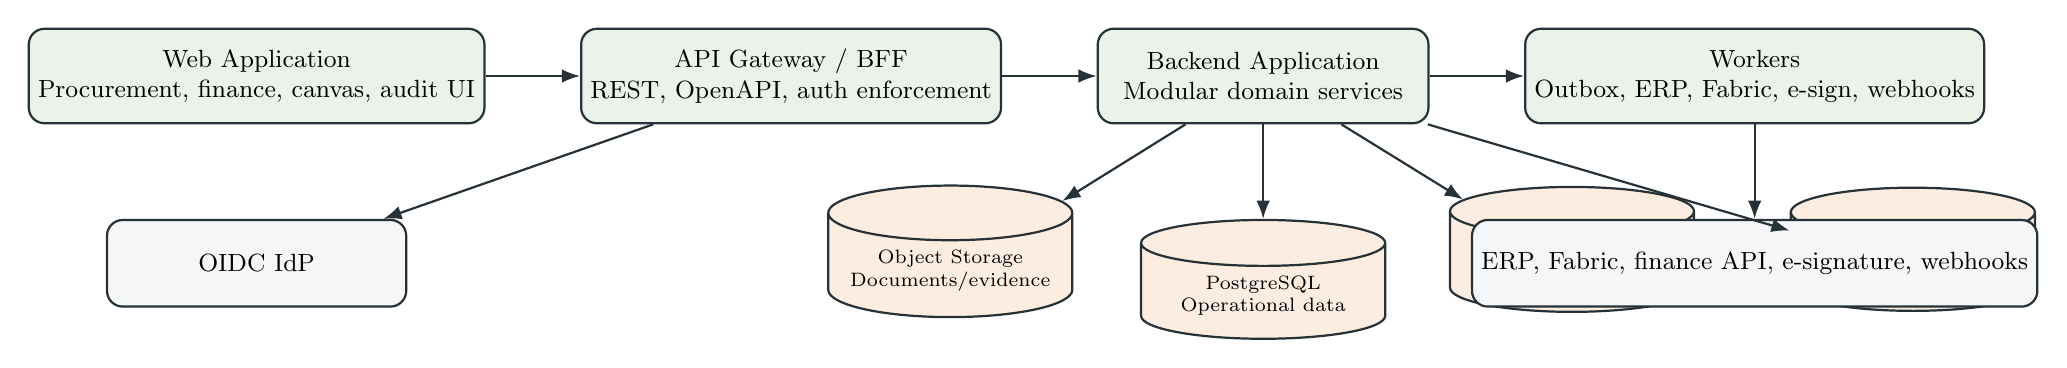
\begin{tikzpicture}[node distance=12mm]
\node[c4container] (web) {Web Application\\Procurement, finance, canvas, audit UI};
\node[c4container, right=of web] (api) {API Gateway / BFF\\REST, OpenAPI, auth enforcement};
\node[c4container, right=of api] (backend) {Backend Application\\Modular domain services};
\node[c4container, right=of backend] (worker) {Workers\\Outbox, ERP, Fabric, e-sign, webhooks};
\node[c4database, below=of backend] (pg) {PostgreSQL\\Operational data};
\node[c4database, below left=of backend] (obj) {Object Storage\\Documents/evidence};
\node[c4database, below right=of backend] (redis) {Redis/Queue\\Retry/cache/locks};
\node[c4database, right=of redis] (search) {Search Index\\Optional analytics};
\node[c4external, below=of web] (idp) {OIDC IdP};
\node[c4external, below=of worker] (external) {ERP, Fabric, finance API, e-signature, webhooks};
\draw[c4arrow] (web) -- (api);
\draw[c4arrow] (api) -- (backend);
\draw[c4arrow] (backend) -- (worker);
\draw[c4arrow] (backend) -- (pg);
\draw[c4arrow] (backend) -- (obj);
\draw[c4arrow] (backend) -- (redis);
\draw[c4arrow] (backend) -- (search);
\draw[c4arrow] (api) -- (idp);
\draw[c4arrow] (worker) -- (external);
\end{tikzpicture}
\caption{C4 Level 2 Container diagram}
\end{figure}
\end{landscape}

\section{Key Components and Responsibilities}
\begin{longtable}{L{42mm}L{72mm}L{32mm}}
\toprule
\textbf{Component} & \textbf{Responsibility} & \textbf{SRS} \\
\midrule
Identity and Access & Organization, user, role, workspace scope, API clients, invitations, token claims, permission checks. & \req{FR-01--FR-08} \\
Procurement Core & Requisition, RFQ, quotation, PO, receipt, invoice, matching, contracts, catalogs, spend analytics. & \req{FR-09--FR-24} \\
Supplier/Counterparty & Supplier onboarding, risk documents, Shariah eligibility, bank metadata, performance scores. & \req{FR-19--FR-20} \\
Mudarabah Finance & Opportunity, capital application, due diligence, Shariah review, contract, disbursement, ledger, P/L, closure. & \req{FR-25--FR-42} \\
Policy/Rule Engine & Approval matrix, evidence checklist, financier policy, Shariah checklist, rule versioning. & \req{FR-04,FR-28,FR-30,FR-41} \\
Evidence/Documents & Document metadata, immutable versions, object-store references, hashes, PDF/JSON packs. & \req{DR-04,NFR-23} \\
Audit/Fabric & Append-only audit, canonical hash, Fabric anchor request, transaction reference, verification. & \req{FR-47--FR-50} \\
Graph/Canvas & Nodes, edges, annotations, status/risk overlays, authorization-aware graph views. & \req{FR-43--FR-46} \\
Integration Adapters & ERP, financial entity API, e-signature, CSV/XLSX, webhooks, idempotency, reconciliation. & \req{IR-05--IR-12} \\
Observability/Ops & Health checks, logs, metrics, traces, alerts, backup/restore diagnostics. & \req{NFR-10,NFR-13} \\
\bottomrule
\end{longtable}

\section{Data Model and Data Flow}
\subsection{Data Stores}
PostgreSQL is the transactional source of truth. Object storage holds document payloads, signed artifacts, and evidence packs. Redis/queue infrastructure handles retry state, locks, cache, and background jobs. Fabric stores event hashes and minimal metadata only.

\subsection{Logical Entity Groups}
\begin{longtable}{L{36mm}L{98mm}}
\toprule
\textbf{Area} & \textbf{Entities} \\
\midrule
Identity & Organization, User, Role, Permission, Membership, Workspace, Invitation, APIClient, EmergencyAccessGrant. \\
Procurement & Project, Requisition, RFQ, Quotation, PurchaseOrder, Receipt, ServiceConfirmation, Invoice, PaymentRecord, ProcurementContract, CatalogItem. \\
Mudarabah finance & ProcurementOpportunity, MudarabahApplication, EvidenceChecklist, DueDiligenceReport, ShariahReview, MudarabahContract, Disbursement, ProjectLedgerEntry, ProfitLossStatement, ProfitDistribution, LossException, ClosurePack. \\
Evidence/audit & Document, DocumentVersion, EvidenceItem, EvidencePack, HashRecord, AuditEvent, AuditAnchor, FabricTransactionRef. \\
Graph & NetworkNode, NetworkEdge, VisibilityRule, CanvasView, CanvasAnnotation, RiskOverlay. \\
Integration & ERPMapping, ExternalReference, ReconciliationStatus, OutboxEvent, WebhookSubscription, WebhookDelivery, ImportJob, ExportJob. \\
\bottomrule
\end{longtable}

\subsection{Major Data Flow}
Buyer contract or sales order creates a procurement opportunity. The opportunity generates an evidence checklist and mudarabah capital application. Financier and Shariah reviewers approve or reject. Approved applications generate a restricted contract and e-signature package. Controlled disbursement funds procurement execution. Purchase orders, receipts, invoices, payments, ERP postings, and buyer revenue update the project ledger. Profit/loss is calculated from linked evidence. Closure pack export includes contract, approvals, ledger, distribution/loss decision, audit events, and Fabric anchors.

\section{APIs and Integration Points}
\begin{longtable}{L{36mm}L{58mm}L{42mm}}
\toprule
\textbf{API group} & \textbf{Example endpoints} & \textbf{Purpose} \\
\midrule
Organization & \texttt{/api/v1/orgs}, \texttt{/users}, \texttt{/roles}, \texttt{/workspaces}, \texttt{/api-clients} & Organization and access setup. \\
Procurement & \texttt{/requisitions}, \texttt{/rfqs}, \texttt{/quotations}, \texttt{/purchase-orders}, \texttt{/receipts}, \texttt{/invoices}, \texttt{/matching} & Source-to-pay workflows. \\
Supplier & \texttt{/suppliers}, \texttt{/supplier-documents}, \texttt{/supplier-scores} & Supplier data and performance. \\
Mudarabah finance & \texttt{/opportunities}, \texttt{/applications}, \texttt{/due-diligence}, \texttt{/shariah-reviews}, \texttt{/contracts}, \texttt{/disbursements}, \texttt{/project-ledgers}, \texttt{/profit-loss}, \texttt{/closures} & Financing workflow. \\
Graph & \texttt{/graph/nodes}, \texttt{/graph/edges}, \texttt{/canvas/views}, \texttt{/canvas/annotations} & Network canvas. \\
Audit/evidence & \texttt{/audit-events}, \texttt{/anchors}, \texttt{/verify}, \texttt{/evidence-packs} & Audit and export. \\
Integrations & \texttt{/integrations/erp}, \texttt{/integrations/fabric}, \texttt{/integrations/finance}, \texttt{/integrations/esign}, \texttt{/webhooks} & External systems. \\
\bottomrule
\end{longtable}

External integrations include OAuth/OIDC IdP, ERP/accounting, CSV/XLSX import/export, Hyperledger Fabric Gateway, financial entity API, e-signature provider, and webhook subscribers. All outbound integrations use adapters, idempotency keys, retry state, and reconciliation records.

\section{Security Architecture}
Users authenticate through OAuth/OIDC. Authorization combines organization membership, role, workspace scope, object ownership, object state, and policy conditions. TLS protects all browser, API, ERP, finance API, e-signature, and Fabric gateway traffic. Secrets are held in a secrets store or deployment-approved equivalent. Confidential payloads are stored off-chain; Fabric receives hashes and minimum metadata only.

\begin{longtable}{L{42mm}L{72mm}L{32mm}}
\toprule
\textbf{Threat} & \textbf{Mitigation} & \textbf{SRS} \\
\midrule
Unauthorized financier access & Workspace scopes, graph edge visibility rules, API/service/data authorization, audit denied access. & \req{FR-06,FR-46,NFR-07} \\
Invalid or replayed tokens & Validate issuer, audience, expiry, signature, nonce/scopes, and TLS. & \req{FR-02,NFR-08} \\
Contract tampering & Immutable versions, amendment workflow, hash verification, Fabric anchors. & \req{FR-32,NFR-17,FR-50} \\
Duplicate disbursement & Idempotency, outbox state, external references, reconciliation. & \req{FR-34,NFR-11} \\
Payload leakage to Fabric & Hash-only/minimal metadata default; no full supplier bank details on chain. & \req{DR-05,NFR-18} \\
Lost SME data & Backups, restore tests, migration versioning, object storage backup. & \req{NFR-10} \\
\bottomrule
\end{longtable}

\section{Scalability and Performance Design}
Interactive pages use pagination, server-side filtering, cached reference data, and asynchronous export jobs. Workflow transitions commit local state and audit/outbox events quickly while deferring ERP/Fabric/e-sign/finance API effects to workers. PostgreSQL indexes organization, workspace, status, project, supplier, document number, lifecycle date, and audit correlation IDs. Search indexes and materialized views can support audit search and analytics. Graph/canvas loads filtered visible subgraphs rather than the full network.

\section{Reliability, Availability, Backup, and Disaster Recovery}
The system continues core local procurement when Fabric is unavailable and shows pending-anchor status. ERP, finance API, e-signature, and webhook integrations use retry and idempotency. Backup sets include PostgreSQL, object storage, configuration, secret references, migration version, and integration state. SME self-hosted deployments target RPO 24 hours and RTO 8 hours, matching the SRS.

\section{Deployment Architecture}
Docker Compose is the MVP deployment baseline. Deployment units are reverse proxy, frontend container, backend API container, worker container, PostgreSQL, object storage, Redis/queue, optional search index, and backup job. Helm/Kubernetes is a future managed-deployment option for financial entities or consortium operators.

\section{Observability: Logs, Metrics, Tracing, Alerts}
Logs are structured and include timestamp, service, module, correlation ID, actor, organization/workspace when allowed, event type, and error code. Metrics include request latency, workflow transition duration, queue depth, retry count, database pool state, object store errors, adapter failures, pending anchor age, backup status, and authorization denials. Traces follow requests through API, domain services, database, outbox, workers, and external adapters. Alerts cover high 5xx rate, queue backlog, Fabric anchors stuck, ERP sync failures, object storage failures, and failed backups.

\section{Risks, Assumptions, and Trade-offs}
\begin{longtable}{L{36mm}L{70mm}L{36mm}}
\toprule
\textbf{Risk/trade-off} & \textbf{Implication} & \textbf{Mitigation} \\
\midrule
Mudarabah legal/Shariah variation & Templates differ by institution and jurisdiction. & Configurable templates and human approval. \\
Fabric governance complexity & SMEs may struggle to run peers/orderers/CA. & Managed consortium option and optional anchoring mode. \\
Financial APIs unavailable & Banks/VCs may not expose APIs. & Evidence packs and manual status fallback. \\
Data quality weakness & P/L may be unreliable if procurement evidence is incomplete. & Checklists, validation, ERP reconciliation, auditable waivers. \\
Modular monolith coupling & Boundaries may erode over time. & Module dependency rules, tests, ADRs, extraction criteria. \\
Graph data leakage & Network visibility may expose confidential relationships. & Edge-level access control and scoped read models. \\
\bottomrule
\end{longtable}

\section{Architecture Decisions / ADRs}
\begin{longtable}{L{23mm}L{34mm}L{48mm}L{42mm}}
\toprule
\textbf{ADR} & \textbf{Decision} & \textbf{Rationale} & \textbf{Mapped SRS} \\
\midrule
\adr{001} & Modular monolith for MVP & Easier SME installation and transactional consistency; keep strict bounded contexts for later extraction. & \req{BR-05,NFR-19} \\
\adr{002} & SME-owned node & Supports distributed ownership, data sovereignty, and self-hostability. & \req{BR-05,NFR-21} \\
\adr{003} & PostgreSQL + object storage & Relational workflow state plus scalable document/evidence payload storage. & \req{DR-01--DR-10,NFR-23} \\
\adr{004} & Outbox/idempotency & Prevent duplicate effects and tolerate external failures. & \req{NFR-11,FR-49,IR-06} \\
\adr{005} & OAuth/OIDC + RBAC + workspace scopes & Standards-based identity and controlled financier access. & \req{FR-02,FR-03,FR-06,NFR-08} \\
\adr{006} & Hash-only Fabric anchoring & Tamper-evident audit while preserving confidentiality. & \req{FR-48,DR-05,NFR-18} \\
\adr{007} & Procurement evidence drives finance & Reduces agency risk and profit-verification cost. & \req{FR-25--FR-42,DR-07} \\
\adr{008} & Separate procurement and finance contexts & Distinct lifecycles, rules, and stakeholders. & \req{FR-09--FR-42} \\
\adr{009} & Adapter layer for external systems & Protects domain model from ERP/bank/e-sign variation. & \req{IR-05--IR-12} \\
\adr{010} & Docker Compose first & Practical for SMEs and FYP prototype; Helm later. & \req{NFR-19,NFR-20} \\
\bottomrule
\end{longtable}

\section{Open Questions}
\begin{longtable}{L{22mm}L{88mm}L{32mm}}
\toprule
\textbf{ID} & \textbf{Question} & \textbf{Owner} \\
\midrule
OQ-01 & Which implementation stack will be used for frontend, backend, workers, and migrations? & Technical lead \\
OQ-02 & Which financial entity APIs will be integrated first? & Product owner \\
OQ-03 & What exact Shariah checklist and legal templates are approved for restricted mudarabah contracts? & Shariah/legal advisors \\
OQ-04 & Who operates Fabric peers, orderers, CA/MSP, and chaincode lifecycle in pilots? & Consortium/operator \\
OQ-05 & Which ERP/accounting adapter is first-class in MVP? & Integrator \\
OQ-06 & What retention periods and legal-hold policies apply by jurisdiction? & Compliance \\
OQ-07 & What evidence is sufficient to classify loss as genuine commercial loss versus negligence or breach? & Finance/Shariah/legal \\
OQ-08 & Is PostgreSQL row-level security mandatory for MVP? & Security architect \\
OQ-09 & Which graph/canvas library will be used? & Frontend architect \\
OQ-10 & What plugin sandbox mechanism is required for future extensions? & Architect/security \\
\bottomrule
\end{longtable}

\appendix
\section{Traceability from SRS to Design Decisions}
\begin{longtable}{L{32mm}L{55mm}L{49mm}}
\toprule
\textbf{SRS IDs} & \textbf{Design response} & \textbf{Decision/component mapping} \\
\midrule
\req{BR-01,FR-09--FR-24} & Procurement Core automates source-to-contract and procure-to-pay. & Procurement Core, \adr{001}, \adr{008} \\
\req{BR-02,FR-25--FR-42} & Mudarabah Finance manages application, review, contract, disbursement, ledger, P/L, closure. & Finance Service, \adr{007}, \adr{008} \\
\req{BR-03,DR-07} & Evidence lineage links procurement records, ERP postings, reviewer decisions, and P/L calculations. & Evidence/Documents, Project Ledger, \adr{007} \\
\req{BR-04,FR-30--FR-32} & Policy engine blocks contract generation until financier and Shariah approvals or authorized waivers exist. & Policy Engine, Finance Service \\
\req{BR-05,NFR-19--NFR-21} & SME-owned deployment, Docker Compose baseline, future Helm. & Deployment architecture, \adr{002}, \adr{010} \\
\req{BR-06,FR-06,FR-51} & Bounded opportunity workspaces and invitations. & Identity/Access, \adr{005} \\
\req{BR-07,FR-47--FR-50} & Audit service and Fabric adapter anchor hashes and verify transactions. & Audit/Fabric, \adr{006} \\
\req{BR-08,FR-42,NFR-23} & PDF/JSON closure and evidence packs. & Evidence/Documents, Reporting \\
\req{BR-09,FR-43--FR-46} & Authorization-aware graph/canvas. & Graph/Canvas \\
\req{BR-10,FR-52,IR-01,IR-12} & Versioned APIs, webhooks, extension registry. & API Gateway, Integration, Extension Registry \\
\req{NFR-01--NFR-04} & Pagination, indexing, async workers, optional search. & Scalability/performance design \\
\req{NFR-05--NFR-09} & TLS, secrets, data isolation, token validation, append-only audit. & Security architecture \\
\req{NFR-10--NFR-13} & Backup/restore, integration retry, degraded Fabric mode, observability. & Reliability and observability \\
\bottomrule
\end{longtable}

\section{Glossary}
\begin{description}[leftmargin=40mm,style=nextline]
\item[ADR] Architecture Decision Record.
\item[C4] Context, Container, Component, and Code diagram hierarchy for software architecture.
\item[Fabric anchor] Hyperledger Fabric transaction containing event/document hash and minimal metadata.
\item[Mudarabah] Islamic partnership where the capital provider supplies capital and the entrepreneur/operator manages the venture, with profit shared by ratio and genuine loss borne by capital unless breach/negligence/fraud applies.
\item[Outbox] Durable integration event store used for retryable external side effects.
\item[Workspace scope] Authorization boundary for a selected opportunity, project, or cross-organization collaboration area.
\end{description}

\section{References}
\begin{thebibliography}{99}
\bibitem{iso42010} ISO/IEC/IEEE 42010:2011, \emph{Systems and software engineering -- Architecture description}.
\bibitem{ieee1016} IEEE Std 1016-2009, \emph{IEEE Standard for Information Technology -- Systems Design -- Software Design Descriptions}.
\bibitem{arc42} arc42, \emph{Template for software architecture documentation}, uploaded LaTeX template.
\bibitem{c4} Simon Brown, \emph{The C4 model}, uploaded slide deck.
\bibitem{adrnotes} Richard Thomas, \emph{Architectural Decision Records}, uploaded lecture notes.
\bibitem{srs} \emph{Software Requirements Specification: Mudarabah-Enabled Distributed E-Procurement System}, Version 1.0.
\bibitem{procurement} \emph{Inefficiencies in Traditional Procurement and the Performance Impact of Digital Procurement Solutions}, uploaded evidence review.
\bibitem{mudarabahproc} \emph{Understanding the Link between Mudarabah and Procurement}, uploaded conceptual thesis.
\bibitem{mudarabahmalaysia} \emph{Mudarabah Performance Research Report -- Malaysia}, uploaded research synthesis.
\end{thebibliography}

\end{document}
